\documentclass[border=20pt]{standalone}
\usepackage{tikz}
\usepackage{xcolor}
\usepackage[T1]{fontenc}
\usepackage[scaled]{helvet}
\renewcommand{\familydefault}{\sfdefault}
\usetikzlibrary{arrows.meta, positioning, shapes.geometric, calc}

\definecolor{princetonOrange}{HTML}{E77500}
\definecolor{princetonBlack}{HTML}{1A1A1A}
\definecolor{princetonGrey}{HTML}{6B6B6B}
\definecolor{cardBg}{HTML}{F7F7F7}
\definecolor{borderGrey}{HTML}{C9C9C9}

\begin{document}
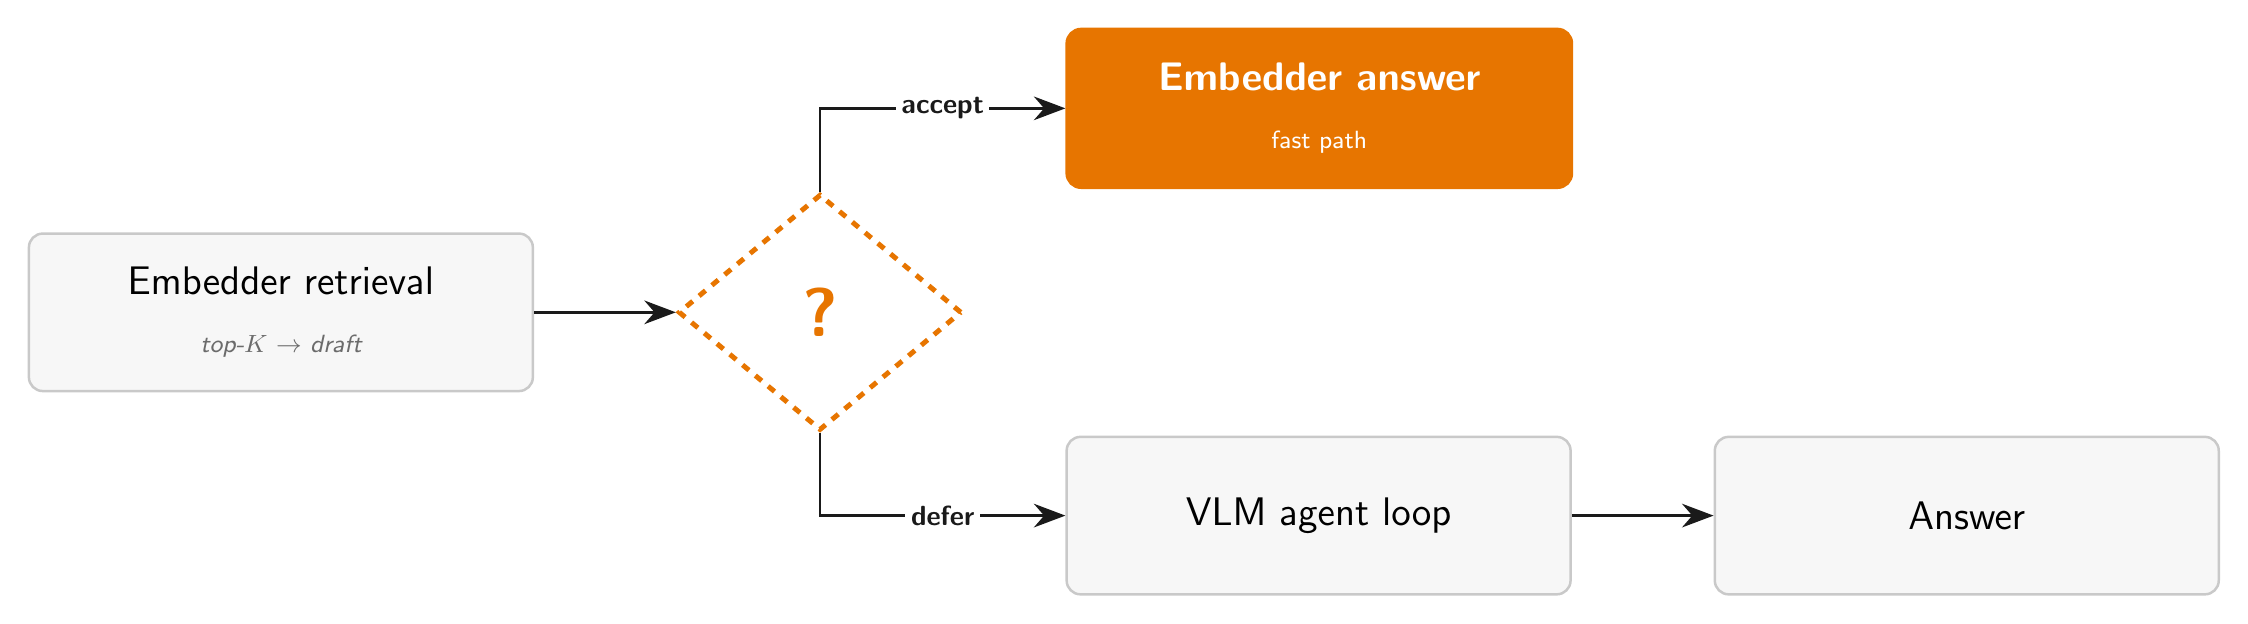
\begin{tikzpicture}[
  every node/.style={font=\sffamily\Large},
  primary/.style={
    draw=borderGrey, line width=0.9pt, fill=cardBg, rounded corners=5pt,
    minimum height=20mm, minimum width=64mm, align=center, inner sep=4mm,
    font=\sffamily\Large
  },
  highlight/.style={
    draw=princetonOrange, line width=1.4pt, fill=princetonOrange, text=white,
    rounded corners=5pt,
    minimum height=20mm, minimum width=64mm, align=center, inner sep=4mm,
    font=\sffamily\Large\bfseries
  },
  opengate/.style={
    draw=princetonOrange, line width=1.8pt, dashed, fill=white,
    diamond, aspect=1.4, align=center, inner sep=2mm,
    font=\sffamily\fontsize{38}{38}\selectfont\bfseries, text=princetonOrange,
    minimum width=36mm, minimum height=30mm
  },
  arrow/.style={-{Stealth[length=4mm, width=3mm]}, line width=1pt, draw=princetonBlack},
  edgelabel/.style={
    font=\sffamily\normalsize\bfseries, fill=white, inner sep=2pt,
    text=princetonBlack
  }
]

\node[primary] (emb) {%
  Embedder retrieval\\[1mm]
  {\sffamily\small\itshape\color{princetonGrey} top-$K$ $\rightarrow$ draft}%
};

\node[opengate, right=18mm of emb] (gate) {?};

\node[highlight, above right=8mm and 22mm of gate] (ans1) {%
  Embedder answer\\[1mm]
  {\sffamily\small\mdseries fast path}%
};

\node[primary, below right=8mm and 22mm of gate] (vlm) {VLM agent loop};

\node[primary, right=18mm of vlm] (ans2) {Answer};

% main flow
\draw[arrow] (emb) -- (gate);
\draw[arrow] (gate.north) |- node[edgelabel, pos=0.75]{accept} (ans1.west);
\draw[arrow] (gate.south) |- node[edgelabel, pos=0.75]{defer} (vlm.west);
\draw[arrow] (vlm) -- (ans2);

\end{tikzpicture}
\end{document}
